%UNLIKE IN A REGULAR TEX FILE, DON'T PUT ANY PREAMBLE MATERIAL HERE

%UNLIKE IN A REGULAR TEX FILE, DON'T PUT ANY PREAMBLE MATERIAL HERE

%%%%%%%%%%%%%%%%%%%%%%%%%%%%%%%%%%%%%%%%%%%%
%\section*{Introduction}
%%%%%%%%%%%%%%%%%%%%%%%%%%%%%%%%%%%%%%%%%%%%

The remarkable technological progress attained in the last few decades has yielded significant benefits in the form of highly advanced imaging, spectroscopic, and polarimetric instruments designed for astronomical observations. These instruments have empowered us with the ability to scrutinize the Sun with exceptional detail. Specifically, the space based observatories have added new avenues of observing sun. Large portions of the electromagnetic spectra is heavily by Earth's atmosphere \sr{Reference here}.  

The studies within this thesis are using solar observations are multi wavelength analysis of solar flares with both imaging and spectroscopy. In this chapter we describe the details of the instruments and techniques used for our analysis.

%%%%%%%%%%%%%%%%%%%%%%%%%%%%%%%%%%%%%%%%%%%%
\section{Solar Dynamic Observatory}
%%%%%%%%%%%%%%%%%%%%%%%%%%%%%%%%%%%%%%%%%%%%

The Solar Dynamics Observatory \citep[SDO;][]{sdo} is a NASA mission designed to understand the causes of solar variability at various spatiotemporal and wavelength scales, as well as its impacts on Earth and the near-Earth environment. It is part of NASA’s Living With a Star program and houses multiple instruments onboard to address its numerous scientific goals. Among the numerous instruments on-board {\it SDO}, we have extensively used data from two instruments – the Atmospheric Imaging Assembly (AIA) and the Helioseismic and Magnetic Imager (HMI).

%%%%%%%%%%%%%%%%%%%%%%%%%%%%%%%%%%%%%%%%%%%%
\subsubsection{Atmospheric Imaging Assembly (AIA)}
%%%%%%%%%%%%%%%%%%%%%%%%%%%%%%%%%%%%%%%%%%%%

AIA \citep{aia} obtains full-disk images of the solar transition region and corona at unprecedented spatio-temporal resolution. The field of view (FOV) covers up to 0.5 $\mathrm{R_{\odot}}$ above the limb. It incorporates several filters at 94 {\AA}, 131 {\AA}, 171 {\AA}, 193 {\AA}, 211 {\AA} and 335 {\AA}, mainly probing the Corona, along with filters at 304 {\AA}, 1600 {\AA}, 1700 {\AA}, and 4500 {\AA}, mainly observing the Chromosphere and Photosphere, providing a total temperature coverage range of 0.06 MK to 20 MK and across various heights. Figure 2.1 illustrates the temperature responses of these filters (Boerner et al., 2012), derived based on the CHIANTI model for solar emissivity (Dere et al., 1997, 2009). Under different conditions, these AIA filters observe different plasma phenomena \citep{o'dwyer10}. Typical exposure times range between 0.5 and 3 seconds. Each AIA telescope is accompanied by its own guide telescope to ensure highly accurate image stabilization. For ous analysis, we have extensively used the coronal EUV channel observations from AIA, e.g. 94 {\AA}, 131 {\AA}, 171 {\AA}, 193 {\AA}, 211 {\AA} and 335 {\AA}. These coronal channels observations are usually available with a 12 s cadence.

%%%%%%%%%%%%%%%%%%%%%%%%%%%%%%%%%%%%%%%%%%%%
\subsubsection{Helioseismic and Magnetic Imager (HMI)}
%%%%%%%%%%%%%%%%%%%%%%%%%%%%%%%%%%%%%%%%%%%%

HMI \citep{hmi} obtains images of the Sun across the \ion{Fe}{1} 6173 {\AA} line at six wavelength locations and infers all four components of the Stokes' parameter. Using these observations, various parameters are inferred e.g., Line of Sight (LOS) magnetic field, Doppler velocities, vector magnetic fields etc. We have mainly used the LOS magnetogram for our analysis. These magnetograms have a 0.5{\arcsec} per pixel resolution and 45 s cadence.

%%%%%%%%%%%%%%%%%%%%%%%%%%%%%%%%%%%%%%%%%%%%
\section{Interface Region Imaging Spectrograph (IRIS)}
%%%%%%%%%%%%%%%%%%%%%%%%%%%%%%%%%%%%%%%%%%%%

The Interface Region Imaging Spectrograph \citep[IRIS;][]{iris} is a NASA small satellite explorer mission designed to observe the dynamics of the lower solar atmosphere. IRIS contains a spectrograph and a slit-jaw imager (SJI), observing the chromosphere, the transition region, and the lower corona. It primarily observes the Sun in two passbands around 1400 {\AA} and 2800 {\AA}. IRIS provides data at high spatial resolution (0.33 {\arcsec} in FUV and 0.4 {\arcsec} in NUV), high time cadence (up to 1 second), and high spectral resolution (12 or 25 m{\AA} per pixel).

IRIS observes three wavelength bands: two in the Far Ultraviolet (FUV) range, spanning 1331.7–1358.4 {\AA} and 1389.0–1407.0 {\AA}, and one in the Near Ultraviolet (NUV) range, covering 2782.7–2851.1 {\AA}. IRIS measures spectra through two primary modes: raster and sit-and-stare. In raster mode, the slit traverses a field of view, capturing spectra from each pixel along its path. When the displacement between consecutive slit positions is comparable to the slit width, it is called dense raster mode; otherwise, it is called sparse raster mode. Alternatively, the instrument may position the slit on a specific region for observation of the Sun. This mode can allow the Sun to naturally rotate across the region or adjust for solar rotation while maintaining continuous observation. This mode is referred to as sit-and-stare. In our analysis, we have used both spectra and SJI imaging from the \ion{Mg}{2} h \& k window and SJI imaging from the \ion{Si}{4} 1402 {\AA} window.

%%%%%%%%%%%%%%%%%%%%%%%%%%%%%%%%%%%%%%%%%%%%
\section{Spectrometer/Telescope for Imaging X-rays (STIX)}
%%%%%%%%%%%%%%%%%%%%%%%%%%%%%%%%%%%%%%%%%%%%

Solar Orbiter \citep[SO;][]{so} is a joint mission between the European Space Agency (ESA) and NASA, launched in February 2020 with the goal of studying the Sun and its dynamic behaviour. The spacecraft aims to provide unprecedented observations of the Sun's polar regions and the inner heliosphere, offering new insights into solar phenomena such as solar wind, coronal mass ejections, and the Sun's magnetic field. We have used observations from the Spectrometer/Telescope for Imaging X-rays (STIX) instrument for our analysis.

 STIX \citep{stix,stix1} is designed to study the Sun's X-ray emissions, providing crucial insights into the processes driving solar flares and other high-energy phenomena. STIX incorporates a set of collimators and detectors to capture high-resolution images of the Sun in X-rays. These images allow scientists to pinpoint the locations and intensities of X-ray emissions associated with solar flares. The instrument covers a broad range of X-ray energies, from approximately 4 to 150 keV, enabling it to observe various aspects of solar activity. STIX can capture X-ray data with high temporal resolution, allowing scientists to study the rapid evolution of solar flares and other transient events in detail. STIX works synergistically with other instruments onboard Solar Orbiter, providing complementary measurements to enhance our understanding of the Sun's dynamic behaviour across different wavelengths and energy ranges.

%%%%%%%%%%%%%%%%%%%%%%%%%%%%%%%%%%%%%%%%%%%%
\section{Extreme Ultraviolet Imager (EUVI)}
%%%%%%%%%%%%%%%%%%%%%%%%%%%%%%%%%%%%%%%%%%%%

Solar Terrestrial Relations Observatory-Ahead \citep[{\it STEREO-A};][]{stereo}, is one of two spacecraft in NASA's STEREO mission, which was launched in October 2006 with the goal of studying the Sun and its dynamic behaviour. {\it STEREO-A} and its twin spacecraft {\it STEREO-B} (Behind) were designed to provide stereoscopic views of the Sun, enabling three-dimensional observations of solar phenomena such as coronal mass ejections (CMEs) and solar flares. Extreme Ultraviolet Imager \citep[{\it EUVI};][]{euvi} is one of the key instruments onboard the {\it STEREO-A} spacecraft. {\it EUVI} is designed to capture images of the Sun in the extreme ultraviolet (EUV) wavelength range. This range of wavelengths is particularly useful for studying the Sun's outer atmosphere, known as the corona, and observing features such as solar flares, coronal loops, and coronal holes. 

{\it EUVI} can capture high-resolution images of the Sun's corona, with spatial resolutions in order of a few arcseconds. It can observe the Sun in 171 {\AA}, 195 {\AA}, 284 {\AA} and 304 {\AA} simultaneously. {\it EUVI} provides continuous observations of the Sun from the STEREO-A spacecraft's vantage point, located slightly ahead of Earth in its orbit around the Sun. This allows {\it EUVI} to monitor solar activity over extended periods and to track the evolution of solar features such as sunspots, flares, and coronal mass ejections (CMEs). We have used 171 {\AA} and 195 {\AA} observations from EUVI for our analysis.

%%%%%%%%%%%%%%%%%%%%%%%%%%%%%%%%%%%%%%%%%%%%
\section{X-Ray Telescope (XRT)}
%%%%%%%%%%%%%%%%%%%%%%%%%%%%%%%%%%%%%%%%%%%%

{\it Hinode} \citep{hinode}, meaning "Sunrise" in Japanese, is a space mission launched by the Japan Aerospace Exploration Agency (JAXA) in collaboration with NASA and the UK Space Agency in September 2006. Also known as Solar-B before its launch, {\it Hinode} is dedicated to studying the Sun's magnetic field and its dynamic behaviour, focusing on understanding the mechanisms driving solar activity and space weather phenomena. The X-Ray Telescope\citep[XRT;][]{xrt} is one of the key instruments aboard the {\it Hinode} spacecraft.

{XRT captures high-resolution solar corona images in X-ray wavelengths, allowing us to study phenomena such as solar flares, coronal loops, etc. Its imaging capabilities enable us to investigate the solar corona's structure, dynamics, and heating mechanisms. XRT utilizes narrow-band filters to isolate specific X-ray emission lines emitted by highly ionized elements in the solar corona. XRT provides continuous observations of the solar corona from the vantage point of the {\it Hinode} spacecraft, which orbits the Earth in a Sun-synchronous polar orbit. This allows XRT to monitor solar activity over extended periods. In our analysis, we used XRT imaging observation from various filters.

%%%%%%%%%%%%%%%%%%%%%%%%%%%%%%%%%%%%%%%%%%%%
\section{Geostationary Operational Environmental Satellites (GOES)}
%%%%%%%%%%%%%%%%%%%%%%%%%%%%%%%%%%%%%%%%%%%%

Geostationary Operational Environmental Satellites (GOES) are a series of weather satellites operated by the National Oceanic and Atmospheric Administration (NOAA) in the United States. These satellites continuously monitor weather conditions across the Americas, including the United States, Canada, Mexico, and parts of South America. GOES data are used by meteorologists and weather forecasters to monitor and predict weather conditions, track severe weather events, and issue warnings and advisories to the public. The continuous monitoring provided by GOES satellites helps improve the accuracy and timeliness of weather forecasts. In addition to monitoring terrestrial weather, GOES satellites also monitor space weather conditions, including solar flares, coronal mass ejections (CMEs), and geomagnetic storms. This information is crucial for forecasting space weather events and assessing their potential impact on satellite communications, navigation systems, and power grids. Among the numerous instruments on-board {\GOES}, we have used data from two instruments extensively {--} X-Ray Sensor (XRS) and Solar Ultra Violet Imager (SUVI).

%%%%%%%%%%%%%%%%%%%%%%%%%%%%%%%%%%%%%%%%%%%%
\subsubsection{X-Ray Sensor (XRS)}
%%%%%%%%%%%%%%%%%%%%%%%%%%%%%%%%%%%%%%%%%%%%

The X-Ray Sensor \citep[XRS;][]{xrs} is an instrument onboard {\it GOES}. The primary function of the XRS is to continuously monitor and measure full disk integrated solar soft X-ray emissions, particularly those associated with solar flares. XRS is designed to detect and measure solar X-ray emissions in two energy bands: short wavelength (0.5 to 4 {\AA}) and long wavelength (1 to 8 {\AA}).

%%%%%%%%%%%%%%%%%%%%%%%%%%%%%%%%%%%%%%%%%%%%
\subsubsection{Solar Ultraviolet Imager (SUVI)}
%%%%%%%%%%%%%%%%%%%%%%%%%%%%%%%%%%%%%%%%%%%%

Solar Ultraviolet Imager \citep[SUVI;][]{suvi} is an instrument aboard {\it GOES}, designed to observe the Sun in the EUV spectrum, providing crucial data for monitoring solar activity and space weather. SUVI captures images of the Sun in 94 {\AA}, 131 {\AA}, 171 {\AA}, 195 {\AA}, 284 {\AA} and 304 {\AA}. These wavelengths are very similar to AIA and provide complementary observations. The FoV of SUVI is rotated by $\sim~45^{o}$, and hence, provides a larger radial distance coverage along the diagonals. In our analysis, we have used SUVI observations from 94 {\AA}, 131 {\AA}, 171 {\AA}, and 195 {\AA}.

%%%%%%%%%%%%%%%%%%%%%%%%%%%%%%%%%%%%%%%%%%%%
\section{Various Plasma Diagnostic Methods}
%%%%%%%%%%%%%%%%%%%%%%%%%%%%%%%%%%%%%%%%%%%%

We employ various techniques throughout this thesis to infer electron density, ion and electron temperature, velocity, thermal structure of the plasma observed in both Chromosphere and Corona. It is standard practice to use atomic databases like CHIANTI \citep{chianti,chianti1} to derive the plasma properties. Below we describe the working principle of the methods used within the scope of this thesis.

%%%%%%%%%%%%%%%%%%%%%%%%%%%%%%%%%%%%%%%%%%%%
\subsection{Differential Emission Measure and Thermal Properties of the Plasma}\label{sec:c2_dem}
%%%%%%%%%%%%%%%%%%%%%%%%%%%%%%%%%%%%%%%%%%%%

Differential emission measure analysis is a commonly employed method with instruments that observe multiple spectral bands to determine the temperature and emission measure of optically thin coronal plasma exhibiting multiple thermal components along a line of sight. However, the inversion process is often challenging due to its ill-posed nature and the frequent lack of sufficient constraints, making it an under determined problem. One of the very first DEM calculation algorithm was {\it xrt\_dem\_iterative}, which was designed and validated for use with XRT data \citep{golub04,weber04}.

The intensity observed by any optically thin imager can be related to the temperature distribution in solar Corona with 
%%%%%%%%%%%%
\begin{equation}
    \mathrm{g_{i}~=~\int_{T}R_{i}(T)~\zeta(T)~dT+\delta g_{i}}
    \label{eqn:dem}
\end{equation}
%%%%%%%%%%%%

In Eqn.~\ref{eqn:dem}, $\mathrm{g_{i}}$ is the counts observed in some specific filter (usually in units of $\mathrm{DN.s^{-1}.pix^{-1}}$), $\mathrm{\delta g_{i}}$ is the observed error, $\mathrm{R_{i}}$ is the temperature response function of the specific filter and DEM(T) describes the thermal distribution of the local plasma  (usually in units of $\mathrm{cm^{-5}.K^{-1}}$). For multiple filter observations, this problem can be posed as a matrix equation in the form of $\Vec{g}~=~\mathbb{R}~\Vec{\zeta}\implies \Vec{\zeta}~=~\mathbb{R}^{-1}\Vec{g}$. However, because of the ill-posed and under-determined nature of the inverse problem, any attempt to invert this set of equations and recovering the DEM results in a significant increase in the noise.

There are several well-characterised methods for inverting the DEM. In this thesis, we have used the method based on regularized inversion developed by \cite{hannah&kontar12}, to infer the thermal distribution of the coronal plasma.Given the under-defined nature of the inverse problem, the problem reduces to a least-square minimizing problem

%%%%%%%%%%%%
\begin{equation}
    \mathrm{||\Tilde{\mathbb{R}}\zeta(T)-\Tilde{g}||^{2}+\lambda||{\bf L}(\zeta(T)-\zeta_{0}(T))||^{2}~=~min}
    \label{eqn:dem}
\end{equation}
%%%%%%%%%%%%

where $\Tilde{\mathbb{R}}~=(\delta g)^{-1}\mathbb{R}$ and $\Tilde{g}~=(\delta g)^{-1} g$. The minimization is performed using the Lagrange multiplier method. {\bf L} is the constrain matrix, $\lambda$ is the regularization parameter and $\zeta_{0}(T)$ is the initial guess solution for the DEM. For further details please refer to \cite{hannah&kontar12}.

With the inverted DEM we get information regarding the distribution of the plasma at a range of temperatures. We can calculate the Emission Measure (EM) given by, $EM=\int_{T}DEM(T)~dT$ (in units of $\mathrm{cm^{-5}}$). The EM is connected to the local plasma density by $EM=\int n_{e}^{2}~dl$. We can also infer the average temperature of the local plasma with the DEM by, $\bar{T}=\frac{1}{EM}\int_{T}DEM(T)~T~dT$.

%%%%%%%%%%%%%%%%%%%%%%%%%%%%%%%%%%%%%%%%%%%%
\subsection{Plasma Velocity from Spectra}
%%%%%%%%%%%%%%%%%%%%%%%%%%%%%%%%%%%%%%%%%%%%

The bulk motion of the plasma along our line of sight can be easily inferred by measuring the red/blue shift of various lines compared to their rest wavelengths. This shift in wavelength is related to the LOS velocity by, $\frac{V_{LOS}}{c}~=~\frac{\Delta \lambda}{\lambda}$.

In addition to the plasma's bulk velocity, several parameters can be inferred from the spectra. The spectral lines are formed due to the transition of electrons between two atomic/ionic energy levels. Instead of a sharp Dirac-delta function, we get the spectra broadened over a wavelength range due to several factors, {\it e.g.}, thermal broadening, Doppler broadening, pressure, optical depth, etc. The FWHM of the spectral line is given by, $\mathrm{FWHM~\sim~\frac{\lambda_{0}}{c}\sqrt{\frac{2k_{B}T}{m}+v_{nth}^{2}+r^{2}}}$. Here, $\lambda_{0}$ is the central wavelength, T is the temperature of the plasma, m is the mass of the ion, $\mathrm{v_{nth}}$ is the non-thermal velocity and r is the given instrumental width. 

The non-thermal broadening of spectral lines is caused by various factors {\, e.g.}, turbulence, wave motion, nano flares, small-scale local flows, magnetic reconnection, etc. All of these broadening appear on top of the Doppler broadening. Accurate estimation of the non-thermal broadening depends significantly on the accurate estimation of the instrumental broadening.

%%%%%%%%%%%%%%%%%%%%%%%%%%%%%%%%%%%%%%%%%%%%
\section{The Solar Ultraviolet Imaging Telescope}
%%%%%%%%%%%%%%%%%%%%%%%%%%%%%%%%%%%%%%%%%%%%

Numerous modern and historical imaging, spectroscopic, and polarimetric instruments have significantly contributed to our comprehension of the Sun and its atmosphere. Several of these instruments, previously discussed, have been utilized in this thesis. While certain instruments are ground-based telescopes, others operate from space. Space-based instruments primarily observe the Sun in Ultraviolet (UV), extreme ultraviolet (EUV), and X-ray bands, capturing radiation emitted from upper atmospheric layers like the transition region and corona, which possess elevated temperatures. Over recent decades, various studies of the Sun have effectively unveiled the physical characteristics of the gas in its upper atmospheric layers using observations recorded by X-ray imaging (e.g., {\it Hinode} X-ray Telescope \citep[{\it Hindoe}/XRT,][]{xrt}) and spectroscopy (e.g., the Spectrometer/Telescope for Imaging X-rays on {\it Solar Orbiter} \citep[{\it SO}/STIX,][]{stix}) as well as extreme ultraviolet (EUV) imaging (e.g., Atmospheric Imaging Assembly on the {\it Solar Dynamic Observatory} \cite[{\it SDO}/AIA,][]{aia}; Extreme ultraviolet Imaging Telescope on {\it Solar and Heliospheric Observatory} \cite[{\it SoHO}/EIT,][]{eit}; Solar Ultraviolet Imager on the {\it Geostationary Operational Environmental Satellites} \citep[{\it GOES}/SUVI,][]{suvi}; the Extreme Ultraviolet Imager on {\it Solar Terrestrial Relations Observatory-A} \cite[{\it STEREO-A}/EUVI,][]{stereo,euvi}; the Extreme-Ultraviolet Imager on {\it SO} \citep[{\it SO}/EUI][]{eui}) and spectroscopy (e.g., \citep[Hinode/EIS,][]{eis}), among others. Instruments such as the {\it Transition Region and Coronal Explorer} \citep[{\it TRACE},][]{trace}, the Solar Ultraviolet Measurements of Emitted Radiation on {\it SoHO} \citep[{\it SoHO}/SUMER,][]{sumer}, and {\it Interface Region Imaging Spectrograph} \citep[{\it IRIS},][]{iris} have facilitated detailed examinations of the chromosphere and the transition region. These missions offer continuous full-disk and Region of Interest (RoI) coverage of the Sun across X-ray and EUV wavelengths. However, the scenario is notably different in the Near-Ultraviolet (NUV) regime, where there is evidently a lack of continuous full solar disk coverage within this wavelength range.

A significant challenge in conducting solar observations in the UV range from the ground is the substantial attenuation caused by the Earth's atmosphere. To overcome this obstacle, one of the pioneering approaches involved the deployment of stratospheric balloon-borne instruments in 1970 and 1971, as documented by \cite{herse79}. This instrument featured a 20 cm telescope capable of imaging the Sun within the 200-460 nm range. Subsequently, the Rasolba balloon experiment utilized a 30 cm telescope equipped with an ultraviolet spectrograph, yielding high-resolution spectra of the Sun spanning 190 to 295 nm \citep{samain85,staath95}. Building upon these endeavors, the Sunrise project \citep{sunrise1,sunrise2} emerged as a balloon-borne observatory designed to observe the Sun in the Near Ultraviolet (NUV) range using a 1 m diameter telescope. Sunrise conducted two flights, in June 2009 and June 2013, respectively, and provided high-resolution imaging at wavelengths of 214, 300, 312, 388, and 397 nm with the Sunrise Filter Imager \citep[SuFI,][]{sufi} in 2009, and at 214, 279, and 397 nm in 2017 \citep{sunrise2}. Additionally, Dopplergrams and vector magnetograms were obtained in \ion{Fe}{1} 525.02 nm using the Imaging Magnetograph eXperiment \citep[IMaX,][]{imax} at various locations on the solar disk. Throughout these flights, Sunrise observed a variety of solar phenomena, including emerging flux events \citep{centeno17}, properties and dynamics of moving magnetic features around pores \citep{kaithakkal17}, proper motion of bright points in quiet sun and active regions \citep{jafarzadeh17}, and properties of fibrils \citep{gaferia17}. These observations underscored the wealth of information carried by this wavelength range and paved the way for full-disk coverage of the Sun in the NUV.

The Solar Ultraviolet Imaging Telescope \citep[SUIT;][]{ghosh16,article}, iss one of the seven payloads aboard the Aditya-L1 mission \citep{adityal1, aditya} led by the Indian Space Research Organization (ISRO). Launched on September 2, 2023, the satellite orbits around the Sun-Earth L1 point in a halo orbit. Equipped with eleven science filters, comprising eight narrow band and three broad band filters, SUIT possesses a distinctive capability to explore various heights within the solar photosphere and chromosphere. This capability aids in understanding the diverse physical processes involved in the transport of mass and energy across different layers of the Sun. Additionally, SUIT offers a unique opportunity to spatially measure the solar spectral irradiance in the Near Ultraviolet (NUV) range, a critical aspect in advancing our comprehension of Sun-climate relationships.

{\suit} is designed to deliver continuous full-disk and Region of Interest (RoI) solar images, boasting a plate scale of 0.7 \arcsec. It possesses the ability to track RoIs while compensating for the effects of differential rotation, as outlined by \cite{suit_algo}. Additionally, SUIT is equipped with onboard intelligence to detect and localize flares, and it can autonomously adjust exposure times to prevent saturation. The primary scientific inquiries targeted by SUIT include \citep{suit_science, suit_main}:

\begin{itemize}
    \item dynamic coupling between the lower and the middle solar atmosphere
    \item measurement of solar spectral radiance in the NUV.
    \item spectral energy distribution of solar flares in NUV
    \item dynamics of chromospheric eruptive phenomena at various spatiotemporal scales
    \item Initiation of Coronal Mass Ejections(CMEs) and space weather: the kinematics of erupting prominences during the early phase.
\end{itemize}

%%%%%%%%%%%%%%%%%%%%%%%%%%%%%%%%%%%%%%%%%%%%
\subsection{SUIT \& Solar Flares}\label{sec:suit_and_flare}
%%%%%%%%%%%%%%%%%%%%%%%%%%%%%%%%%%%%%%%%%%%%

Solar flares are the most powerful magnetic events in the solar system. They are described as a sudden increase in brightness in localized areas on Sun. Within tens of minutes, they can release over $10^{32}$ erg of energy, which is emitted across the entire electromagnetic spectrum from radio to gamma rays. They can also launch high energetic particles into the interplanetary medium. Most of the flares occur in magnetic active regions, and the amount of flare energy released is comparable to the free energy stored in the magnetic system. The term "flare" is generally used explicitly for the entire magnetically-driven event's electromagnetic radiation, as it is the most significant fraction of the total energy liberated. The total energy released varies from event to event. It is also known that larger events occur much less frequently than smaller events.

The Solar Ultraviolet Imaging Telescope \citep[SUIT;][]{ghosh16,article} is one of the seven payloads onboard the Aditya-L1 mission \citep{adityal1} of the Indian Space Research Organization (ISRO). With its 11 science filters (3 broadband and eight narrowband), SUIT will have the capability to probe different heights of solar atmosphere in photosphere and chromosphere to help us understand the various processes that transport mass and energy from one layer to another. SUIT will provide full disk as well as partial disk images of the Sun with a pixel size of 0.7". Through SUIT imaging, we would be able to resolve solar flares spatially on the surface of the Sun, for the first time in near ultra-violet (NUV), which will help us to address the questions regarding their build-up and triggering mechanism. In addition, to measure the spatially resolved solar spectral irradiance within the wavelength range that is central for studying the Chemistry of oxygen and ozone in the Stratosphere of Earth's atmosphere.

It has been shown that the majority of flare energy emerges at the visible and UV wavelength range \citep{woods06}. \cite{woods04} showed that about 77\% of the energy is released in the wavelength range > 200 nm, and only ~ 23\% is seen in extreme ultraviolet (EUV) and soft X-ray (SXR), i.e., below 200 nm \citep{Nei_1989,neidig93,kretzschmar11}. Although the energy content in hard X-ray (HXR) is a tiny fraction of the total energy budget, they are still crucial in understanding the energization process \citep{holeman11}. However, to develop a comprehensive understanding of solar flares, it is mandatory to perform multi-wavelength studies of all kinds of flares. This may have implications on the physics of the origin of solar flares and different physics processes and contribute to the solar spectral irradiance as a function of the solar activity cycle. Although we have been observing Sun and Solar flares in various wavelengths, the spectral energy distribution of the radiated energy from the flares is still very poorly understood. The first solar flares were observed from the ground in the visible domain \citep{carrington1859,neidig93}. It is also well known that the flare emission in the visible domain occurs mainly in $H\alpha$ and Ca \Romannum{2} lines \citep{canfield90,falchi92,heinzel94}. However, the lesser understood component of the visible and Near Ultra Violet (NUV) emission is the enhancement of the continuum. The study of the white-light (WL) flares has proven to be very difficult because they have a very short duration and low contrast against the background, making their observation from Earth rare and of poor quality. Also, the flares in NUV are not observable from any ground-based instrumentation as most of the NUV gets absorbed in the upper atmosphere, thus requires space-based observations.

The origin of the WLFs, i.e., the physical process responsible for generating the continuum and its contribution to the overall energy distribution, is still highly uncertain. The question remains whether WLFs are photospheric phenomena due to $H^{-}$ free-free emission or chromospheric phenomena due to H free-bound emission. The more recent studies further constrain the origin of the WLFs to be Chromospheric phenomena, as it has been shown that the WL and HXR footpoint centroids are cospatial. Similarly, \cite{krucker15} constrained the cospatial WL and HXR footpoints within the chromosphere for three flares. With the help of SUIT, we would be able to localize the WL flares and resolve them on various parts of the Solar disk, which along with observations from Interface Region Imaging Telescope (IRIS), Helioseismic and Magnetic Imager (HMI), would help us localize the source of the WL footpoints and also comment on the formation mechanism of the WL itself.

\begin{figure}
    \centering
    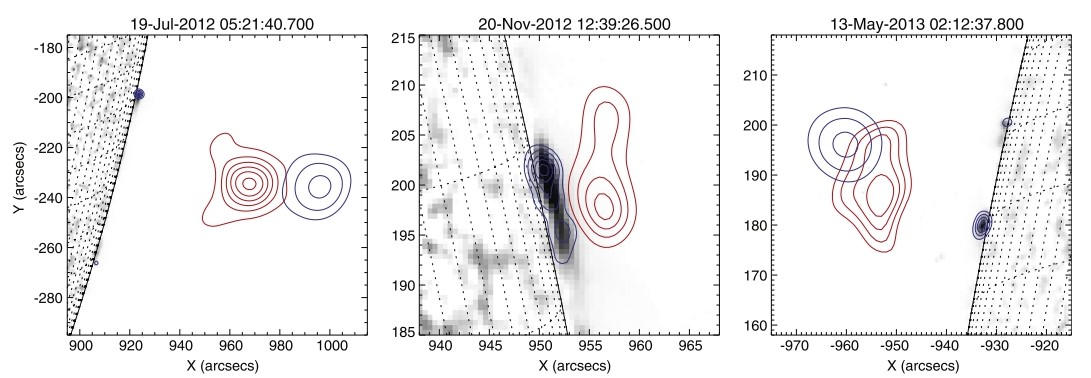
\includegraphics[width = \linewidth]{Figures/Krucker_2015_ApJ_802_19_page-0004.jpg}
    \caption{X-ray and optical imaging of the three flares at the peak time of the impulsive phase: the images are from HMI with the pre-flare image subtracted. The contours represent RHESSI Clean maps in the thermal (red, 12–15 keV) and non-thermal (blue, 30–80 keV) HXR range \citep{krucker15}.}
    \label{fig1}
\end{figure}

The spectral energy distribution of flares is one of the critical areas of interest in the physics of flares. A complete understanding of this will help us decode the physical processes involved in solar flares and help quantify their effects on solar spectral irradiance. Ideally, it would be essential to observe flares at all wavelengths simultaneously with sufficient spatiotemporal resolution to figure out the spectral energy distribution of flares. Unfortunately, this is generally not the case, and we have to rely on the sporadic observations made using ground-based instruments in the visible domain. As mentioned earlier, the majority of the flare energy is emitted in the NUV and visible domain. \cite{kretzschmar10,kretzschmar11}, performed statistical studies using a large number of flare observations across a wide energy range. They demonstrated, at the peak of the flare, about 70\% of the total energy was radiated in the continuum visible and NUV channel as illustrated in \ref{tab1}. SUIT would observe and resolve the solar flares within 200-400 nm using 8 NBs and 3 BBs. This, along with IRIS data, would help us comment on the energy distribution of flares of various classes.

%%--------------------------------------------%%
\begin{table}[]
    \centering
    \resizebox{\textwidth}{!}{%
    \begin{tabular}{||m{.1\linewidth}|m{.15\linewidth}|m{.17\linewidth}|m{.17\linewidth}|m{.17\linewidth}|m{.15\linewidth}||}
    \hline
    \hline
        Mean X-ray class & TSI(ergs) & Ratio $\frac{26-34nm}{TSI}$ & Ratio $\frac{0-50nm}{TSI}$ & Ratio $\frac{0.1-0.8nm}{TSI}$ & Ratio $\frac{continuum}{TSI}$\\
        \hline
        X3.2 & 5.9$\times~10^{31}$ & 0.9-0.8\% & 12-9\% & 1.2-1\% & 67\% \\
        M9.1 & 1.6$\times~10^{31}$ & 1.7-0.4\% & 23-5\% & 1-0.4\% & 85\% \\
        M4.2 & 1.3$\times~10^{31}$ & 2.2-0.5\% & 18-6\% & 0.6-0.3\% & 74\% \\
        M2.0 & 5.1$\times~10^{30}$ & 1.7-0.6\% & 18-6\% & 0.7-0.4\% & 69\% \\
        C8.7 & 3.6$\times~10^{30}$ & 1.5-0.5\% & 16-5\% & 0.4-0.2\% & 72\% \\
        \hline
    \end{tabular}}
    \caption{Spectral Energy Distribution from a sample of 2100 flares across various wavelengths\citep{kretzschmar11}.}
    \label{tab1}
\end{table}
%%--------------------------------------------%%

Finally, one of the major question of interest is how the Solar flares affect the Spectral Solar Irradiance (SSI) and Total Solar Irradiance (TSI) variability from a short to much longer, Solar Cycle timescale. \cite{kretzschmar10,kretzschmar11} performed statistical studies using a large number of flare observations across a wide energy range. For this purpose, they used the full Sun observations of Solar flux from Solar and Heliospheric Observatory (SoHO), three visible Solar irradiances from VIRGO/Solar Photometer (SPM) passbands centred on 402 nm, 500 nm, and 862 nm, respectively, from 1996 to 2008. Additionally, they also use the EUV irradiance in the ranges 0.1-50 nm and 26-34 nm measured by SOHO/Solar EUV Monitor \citep{judge98} and SXR measurements from GOES satellites. They showed that stacked TSI variation profiles during solar flares show variation at more than 2 sigma level during the peak flare time, indicating the presence of flare signals in the TSI measurements.

\begin{figure}[h!]
    \centering
    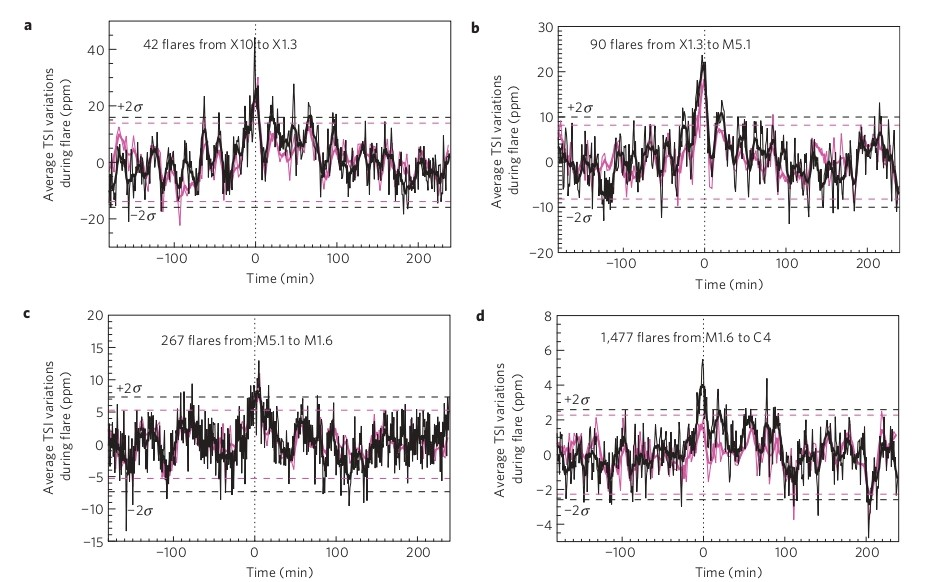
\includegraphics[width = \linewidth]{Figures/nphys1741_page-0002.jpg}
    \caption{Averaged TSI variations during flares. The TSI time-series averages over four exclusive sets of solar flares of decreasing amplitude. The black and pink curves correspond respectively to the TSI measured by the PMOV6 and the DIARAD radiometers. The dashed lines correspond to the 95\% confidence levels, while the vertical line denotes the peak time of the flare \citep{kretzschmar10}.}
    \label{fig2}
\end{figure}

This allows us to quantify the solar variability induced be solar flares of various timescales. With the help of SUIT, we would be able to localize the flare locations and study the change in SSI from the local environment in the 11 science filters. This information combined with TSI measurements can allow us to quantify the effect of flares of various energy scales on the TSI variability of the Sun. As, both the TSI and SSI variability directly or indirectly couples with various atmospheric parameters, we can also study the effect the flares have on them. For example, the Earth's atmospheric chemistry and composition respond to any changes in solar UV output in a very nonlinear fashion \citep{haigh07}. Since the number of flares also shows a change with solar activity, it is prudent to ask how much flares contribute to the solar spectral irradiance in NUV. This is particularly important because the irradiance in NUV plays a key role in heating the upper and middle layers of the Earth's atmosphere directly and their coupling with the Stratosphere. It also directly influences the middle and lower atmosphere chemistry and composition via the Ozone-Oxygen cycle.

%NOTE THE LACK OF A BIBLIOGRAPHY CALL IN THIS FILE. BIBLIOGRAPHY WORK HAPPENS OUTSIDE THE CHAPTER TEX FILES.

%NOTE THE LACK OF A BIBLIOGRAPHY CALL IN THIS FILE. BIBLIOGRAPHY WORK HAPPENS OUTSIDE THE CHAPTER TEX FILES.